\section{Materials And Methods} \label{materials}

\subsection{Creation Of Data From Previous Projects}
This section describes the creation of the dataset and the generation of the force field energies used as the starting point for this thesis. This was initially done in the NetTCR-2.0 paper and Meitil's master thesis \cite{Montemurro2021NetTCR-2.0Data, Meitil2021UsingPrediction}.

\subsubsection{Initial Creation Of Dataset} \label{alessandro_data}
The data originates from paired \acs{cdr}3{\textalpha} and \acs{cdr}3{\textbeta} datasets used by Montemurro et al. The data was initially created as described below \cite{Montemurro2021NetTCR-2.0Data}.

Three sources of data were used to create this dataset.

Positive data was retrieved from VDJdb \cite{Bagaev2020VDJdbCompendium} on the 5th of August 2020, and  IEDB \cite{Vita2015The3.0} on the 26th of August 2020. The negative data was extracted from the 10x dataset \cite{10XGenomics2019APhenotype}. The IEDB and VDJdb contains curated data obtained from published literature, while the 10x dataset was created from single-cell immune profiling of four different healthy humans. The positive TCRs were restricted to only include TCRs with CDR3 lengths between 8-18 that bind peptides with length 9 displayed on HLA-A02*01. 

The negative data was similarly restricted to TCRs with length 8-18 and peptides with length 9. The negatives were identified as TCRs with an Unique Molecular Identifier (UMI) count of 0 for all peptides in the dataset. The UMI count for a given TCR-pMHC data point specifies the number of TCRs with that sequence was bound to the pMHC complex with that UMI.

Redundancy reduction was performed to reduce information leakage between partitions and reduce the amount of redundancy present in the dataset. The positive and negative data were reduced separately using the Hobohm 1 algorithm \cite{Hobohm1992SelectionSets} with 95\% similarity cutoff using the Levenshtein similarity metric \cite{Montemurro2021NetTCR-2.0Data}. The average similarity of the CDR3{\textalpha} and CDR3{\textbeta} was used as the metric for similarity between TCRs. This ensured that no two data points were more than 95\% similar within their class. The positives were then randomly partitioned into 5 partitions, and the negatives were added randomly in a 3:1 ratio to the 5 partitions.

\subsubsection{Adding Swapped Negatives}
Swapped negatives were added to force the model to learn what specific peptides the TCR binds instead of only identifying what makes a positive TCR. The swapped negatives were generated by taking a positive TCR and selecting a different random peptide from the same partition. The swapped negatives were kept in the same partitions as the positive TCR to avoid information leakage.

\subsubsection{Retrieval Of V Gene Sequence And Force Field Modelling}
Recreating the entire TCR sequence and the force field modelling was done by Meitil in her thesis \cite{Meitil2021UsingPrediction}. The negatives from the 10x dataset already had an annotated V gene, which could be used to recreate the missing sequence. For the positive CDR3s, they were mapped to the VDJdb to retrieve the V gene. 

The hidden markov model from LYRA \cite{Klausen2015LYRAModeling} was used to align the V gene sequence with the CDR3 to form the whole TCR sequence.

TCRpMHCmodels was used to estimate a TCR-pMHC structure used for the energy calculations \cite{Jensen2019TCRpMHCmodels:Complexes}. The resulting PDB files were used to create force field simulations of interaction energies using Rosetta and FoldX \cite{Schymkowitz2005TheField, Alford2017TheDesign}. Rosetta generated both interaction energies for each residue in the sequence and global interaction terms between the proteins. FoldX was used to add additional global interaction terms between the proteins. See the thesis by Meitil for specific commands used to generate interaction energies \cite{Meitil2021UsingPrediction}.

TCRpMHCmodels succeeded in generating a structure for 82.9\% of the positive complexes and 97\% of the negative \cite{Meitil2021UsingPrediction}. The total amount of data points ends up at 6897 (1721 positives, 1721 swapped and 3455 negatives).

\subsection{Creation Of Comparable CDR Dataset}
To investigate the relevance of the energy features on only the CDR3{\textalpha} and CDR3{\textbeta}, the per residue energy features simulated using Rosetta would have to be restricted to only these sequence features. The sequences created with LYRA had not been annotated after construction. Therefore, IgBLAST \cite{Ye2013IgBLAST:Tool.} was used to annotate the full TCRs, and afterwards, the per residue energy features were restricted to the CDR3 positions.

\subsection{Constructing Input For Networks}

The amino acid sequence had to be encoded or embedded in a representation useable by the network. Encoding of the data was done using a BLOSUM50 matrix scaled by a factor of $\frac{1}{5}$. A vector of length 20 is created for each residue, yielding an l x 20 matrix for a sequence with length l. The other approach creates embeddings using a Word2Vec model for the CDR3 sequences and is explained in Section \ref{embedding}. Not all TCR sequences have the same length. Therefore, the sequences were padded on the right with zeros such that all TCR{\textalpha}/CDR3{\textalpha} and TCR{\textbeta}/CDR3{\textbeta} had the same length. The sequence encoding was combined with the energy features generated by Rosetta and FoldX.

The dimensions of the final tensor used for training can be seen in Figure \ref{fig:data_tensor}. Each of the 6897 TCRpMHC complexes is a matrix with the padded sequences as the first dimension and the encoding and energy features as the second dimension.
\begin{figure}[H]
    \centering
    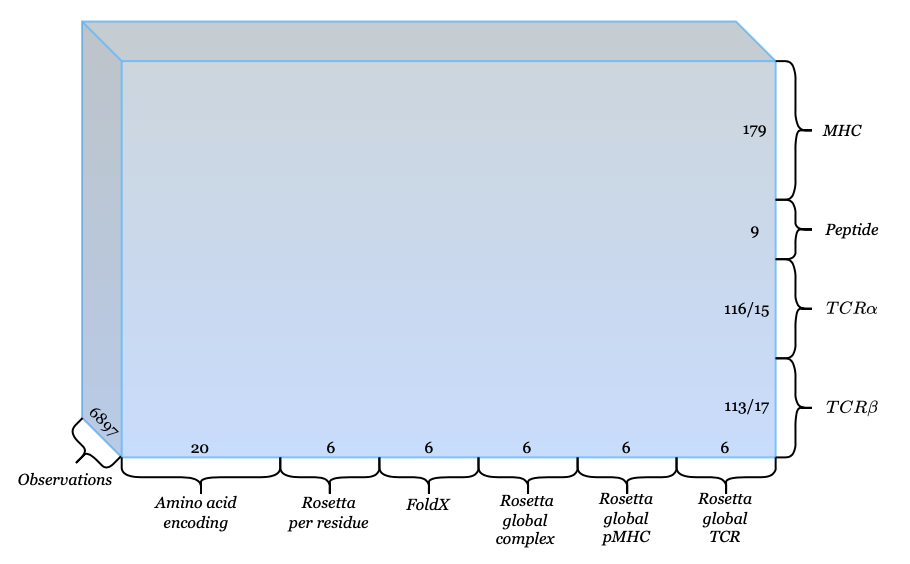
\includegraphics{figures/data_figure.png}
    \caption{Dimensions of dataset used throughout the project. TCR{\textalpha} and TCR{\textbeta} shows dimensions for full TCR and only CDR3 respectively.}
    \label{fig:data_tensor}
\end{figure}

\subsection{Downsampling of Dataset}
The full dataset still contains some level of redundancy even with the Hobohm redundancy reduction using Levenshtein similarity. Two different types of partitions were created. One to investigate how the model performs when redundancy is reduced further, and the other to see what happens when the amount of training data becomes limited. The first approach is similar to the approach used for data creation using Hobohm 1. The other uses random sampling to be able to subsample peptides individually.

\subsubsection{Kernel similarity} \label{kernel_sim}
Multiple datasets were created with a decreasing amount of redundancy. The approach used here is modified from the approach described in Section \ref{alessandro_data}. Here a kernel similarity using k-mers \cite{Shen2012TowardsChains} was used instead of the Levenshtein similarity as the similarity measure for the Hobohm 1 cutoff. The kernel calculates the similarity between two sequences without an alignment. The similarity is calculated using the BLOSUM62 matrix to compare all k-mers generated from the two sequences, with k being all integers in $k\in[1, 30]$. The kernel also uses the BLOSUM62 matrix to compare amino acids from the k-mers. The similarity is averaged over the CDR3{\textalpha} and CDR3{\textbeta} to obtain an overall similarity for the TCR. 

The kernel similarity gives a value between 0 and 1, where a high value means high similarity, which is used by the Hobohm algorithm to reduce redundancy. After obtaining a list of less redundant positives and negatives, they were randomly distributed to 5 partitions as before. The swapped negatives were dealt with differently. If a positive TCR was removed during the Hobohm 1 redundancy reduction, the swapped negatives generated from the removed positive TCR were also removed from the dataset. Else the swapped negative was added to the same partition as the corresponding positive TCR.

This was repeated for several similarity cutoffs (1, 0.98, 0.95 and 0.9), which yielded datasets with a decreasing number of observations (6897, 6345, 5698, 4534, respectively).
\subsubsection{Random Sampling} \label{subsample}
A single peptide was randomly downsampled to create smaller datasets and investigate performance when training data for a single peptide is limited. Sampling was done stratified by downsampling each type of sequence (positive, swapped negative or 10x negative) individually from the primary dataset. The sampling was done for a single peptide while keeping all observations from the other peptides. If a positive TCR was removed, the swapped negative TCRs were also removed. This type of sampling simulates a situation where model performance on a single peptide can be seen as a function of the number of TCRs for that specific peptide, as opposed to the kernel similarity method, where all peptides were downsampled.

\subsection{Network Architectures}

\subsubsection{Convolutional network}
% Find andre typer TCR modeller som CNN og cite
A 1-layer CNN similar to the approach used in NetTCR-2.0 \cite{Montemurro2021NetTCR-2.0Data} was implemented to benchmark against a simplified version of the NetTCR-2.0 model. The architecture can be seen in Figure \ref{fig:cnn_architecture} and consists of parallel convolutional and max pool modules followed by a 1-layer FNN using the output from all the parallel max pools as input.

Each CNN contains 20 convolutional filters with size 3. Each filter contributes one value to the dense input by doing a global max pool. Each type of sequence (MHC, peptide, TCR{\textalpha} and TCR{\textbeta}) has its own set of filters, yielding a total of 120 filters. TCRs were either represented as the whole TCR or restricted to the CDR3. The global max pool means only the three positions in the sequence the filter deems most informative get to contribute to the prediction. The use of multiple filters then allows multiple different types of information to be captured from the sequence and used for prediction. The global max pool is a simple attention mechanism by selecting the highest value and has no learnable weights directly tied to attention. Instead, the convolutional filters are responsible for finding motifs and ensuring the attention is put on the important sections of the sequence. This architecture allows us to model our many-to-one problem by removing the sequence dimension through the global max pool.

The activation function used for the convoluted outputs was the sigmoid function. The dense layer had a size of 64 neurons and used the Tanh function as the activation function for the hidden layer and the sigmoid function on the final output value to shrink it to the interval $\hat{y} \in (0,1)$.

This network was also used to investigate the importance of the different features in the data. Here, the model also uses the MHC and the energy features, which are not used in the LSTM-based models. The global energy features were added after the convolutional layers, as these describe the complex as a whole and do not need max pooling to generate global terms. Certain sequences or features such as the sequence encoding was removed as input during training and evaluation to find the model's most important features and sequences. However, only features used in all models (peptide and CDR3s without any energy features) were used to ensure a legitimate comparison between the different architectures.
\begin{figure}[H]
    \centering
    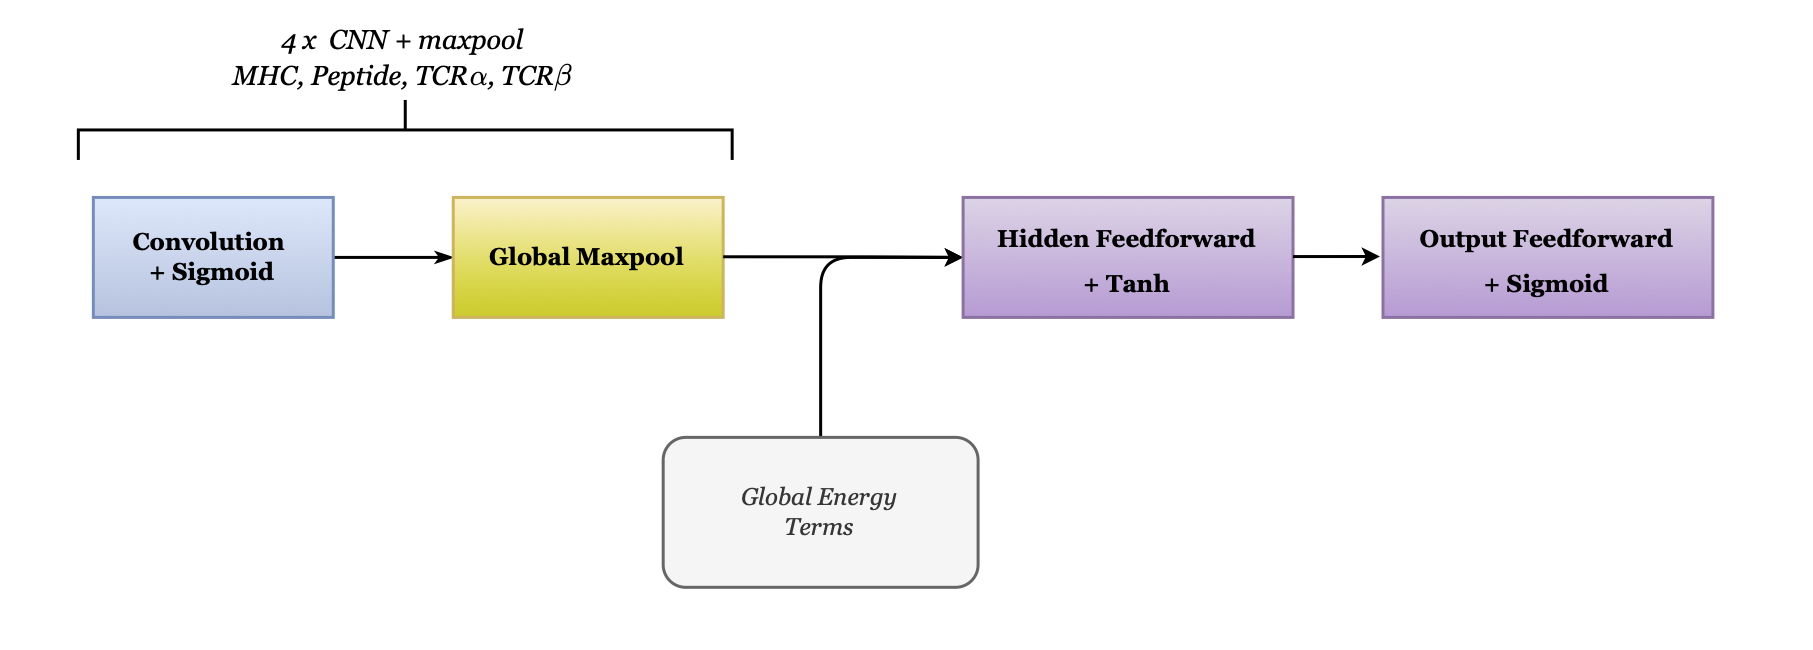
\includegraphics[width=\linewidth]{figures/cnn_architecture.png}
    \caption{CNN model used in this project. The model consists of 4 parallel CNNs for the encoded sequences. The CNN output is concatenated and used as input in a dense layer to generate output predictions.}
    \label{fig:cnn_architecture}
\end{figure}

\subsubsection{LSTM network}
A simple Bidirectional LSTM (biLSTM) network was implemented as a baseline LSTM based neural network. A schematic view of the network can be seen in Figure \ref{fig:lstm_architecture}. Here the different sequences (peptide, CDR3{\textalpha} and CDR3{\textbeta}) are used as input to three parallel biLSTMs. The hidden representation of the biLSTM had a size of 24 for all sequence types. The last hidden state from all three biLSTMs is then concatenated to a vector with 144 ($24 \cdot 3 \cdot 2$) entries and fed into a dense layer using the same activation functions and dimensions as the CNN model.

This architecture should propagate the most important signals through the recurrent network, which is then recovered as the last hidden state. The dense layers are again responsible for generating the prediction. However, the input comes from parallel LSTMs instead of parallel CNNs with global max-pooling.

\begin{figure}[H]
    \centering
    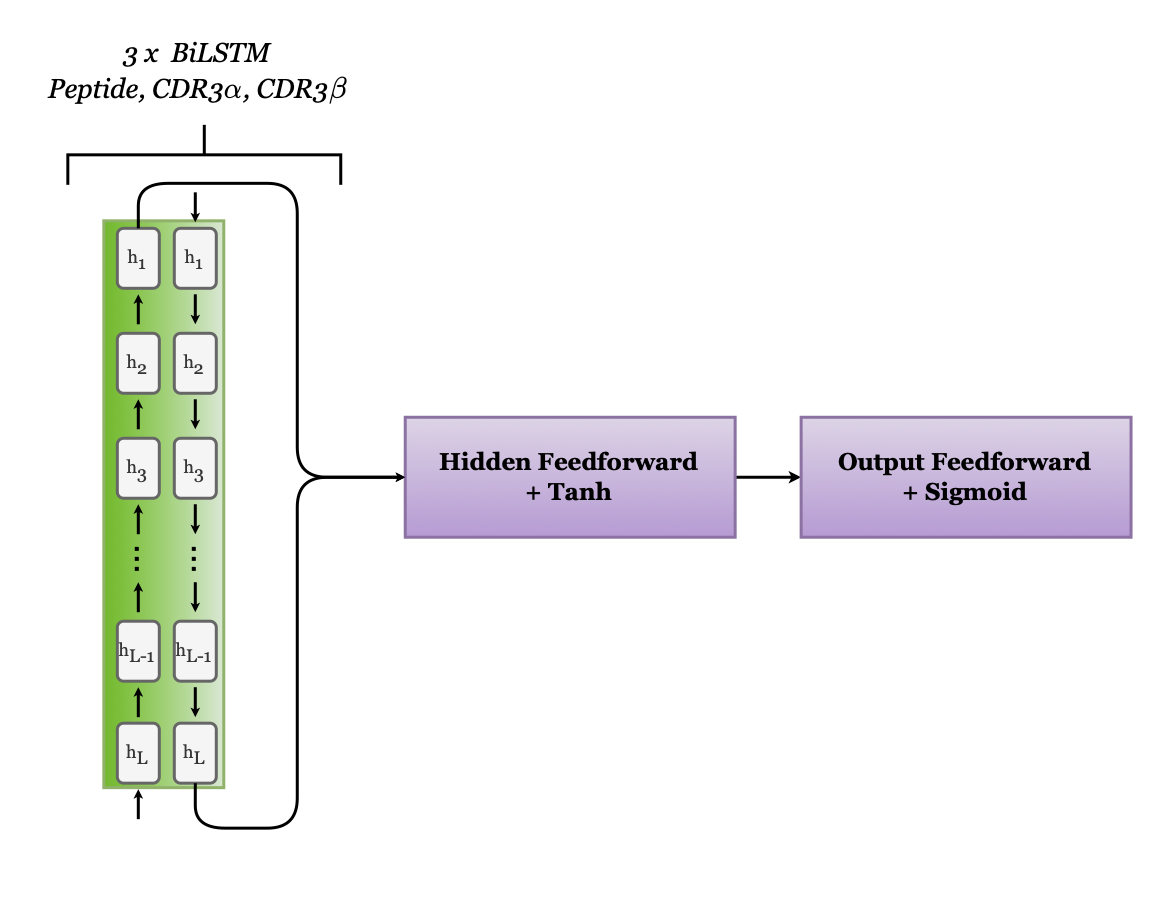
\includegraphics[width=\linewidth]{figures/lstm_architecture.png}
    \caption{LSTM network used in this thesis. The hidden output from each of the directions in the biLSTM is concatenated with the other sequences and used as input for a 1-layer dense network.}
    \label{fig:lstm_architecture}
\end{figure}

\subsubsection{AttLSTM network}
% Cite modeller som bruger attLSTM (Deeploc, den der anden protein halløj)
Attention can create an importance weighted average of the different positions in the sequence and allow hidden states from all positions to contribute to the dense input. The schematic view of this approach is shown in Figure \ref{fig:attLSTM_architecture}. Similarly to the LSTM network each type of sequence (peptide, CDR3{\textalpha} and CDR3{\textbeta}) is passed through a biLSTM. However, instead of extracting the last hidden state, a weighted average of the hidden states for each position is used. The attention layer introduced in Section \ref{section:attention} calculates the weight for each position's hidden state, which is then used to generate a weighted hidden state. 

The hidden dimension in the biLSTM was set to 24 as in the LSTM network. The hidden dimension in the attention layer (number of features in the context vector and hidden representation of the LSTM output, see Figure \ref{fig:attention_schema}) was set to 24. The weighted average of the output states is calculated using matrix multiplication for both directions of the biLSTM and concatenated with the different sequence types, yielding a vector of length 144 as input for the dense layer, which is identical to the previous explained dense layers.

\begin{figure}[H]
    \centering
    \includegraphics[width=\linewidth]{figures/attLSTM_architecture.png}
    \caption{attLSTM architecture. A biLSTM generates an output for each position. Each output is then combined using a weighted average, by using attention to determine the importance of specific positions. The weighted average is concatenated with the output from the other sequences and used as input in a single dense layer.}
    \label{fig:attLSTM_architecture}
\end{figure}

\subsection{Amino Acid Embeddings} \label{embedding}
% ProtVec og andre skal cites her.
Embeddings were generated using the Word2Vec model \cite{Mikolov2013EfficientSpace, Rehurek2011Gensim--pythonModelling}. Due to the low number of unique peptides in our dataset, generating a peptide-specific embedding using Word2Vec is not feasible. However, CDR specific embeddings were created by taking positive non-crossreactive TCRs with specificity towards peptides bound to Human leukocyte antigen (HLA)-A*02:01 from the 10x dataset (n = 9606). The positives were supplemented with 190000 randomly sampled TCRs negative towards peptides from HLA-A*02:01 from the 10x dataset. Additionally, to investigate the ability of Word2Vec to extract information on biophysical properties of amino acids, 20000 sequences were randomly sampled from the Swiss-Prot database \cite{Bateman2021UniProt:2021} and used to train a general protein embedding used only for visualization.

CDR3{\textalpha} and CDR3{\textbeta} embeddings were trained separately using the skip-gram algorithm. After training, the embeddings for each residue consist of a vector with a size of 20. For the peptide sequence, the embedding weights were initialized randomly from $\mathcal{N}(0,1)$. These embeddings are initially used to represent the sequence similar to the approach with BLOSUM encoding. However, the embeddings were updated during model training, thereby fine-tuning them to improve the embeddings and be specific towards predicting TCR-pMHC binding.

\subsection{Training Neural Networks} \label{training}
All networks were implemented in Pytorch 1.10.2 \cite{Paszke2019PyTorch:Library} and Python 3.8.3. All networks were trained using a weighted binary cross entropy.

\begin{equation}
    - \frac{1}{N} \sum_i^N w_i \cdot y_i \cdot \log(\hat{y}_i) + (1-w_i) \cdot (1-y_i) \cdot \log(1 - \hat{y}_i)
\end{equation}
Here N is the number of observations, $w_i$ is the weight on the positive class calculated as the fraction of negatives in the training data, $y_i$ is the class, either 0 or 1, and $\hat{y}_i$ is the prediction for the observation.

The weighted version was introduced to increase the importance of the positive observations in the loss function. Using an unweighted version of cross entropy resulted in the model only predicting the negative class. The Adam optimizer was used to update the weights using a learning rate of 0.005 \cite{KingmaADAM:OPTIMIZATION} and the batch size used was 64. For initialization of the weights, the uniform kaiming was used \cite{https://doi.org/10.48550/arxiv.1502.01852}.

All networks contained dropout layers with a probability of 0.3 before and after the convolutional or LSTM layers and at the hidden dense layer. The dropout was enabled during training and subsequently disabled for evaluation. Early stopping was used with patience set to 10 epochs to avoid overfitting further. If there was no improvement in the loss after the 10 epochs, training was stopped.

Performance evaluation was done using a nested cross-validation approach. One partition was kept as a test set, one was chosen as a validation set for early stopping and three partitions were used for training the model. After training, the test set was predicted using the trained model, and the partitions were reassigned to training, validation and test. After the nested cross-validation, each observation had four predictions. The average of the four predictions was taken to generate a single prediction value.

AUC was calculated using scikit-learn and was calculated primarily only using the positive and true negatives. The swapped negatives were not included unless explicitly stated in the AUC calculations.

%\subsection{Pretraining peptide specific attLSTM model}
%Models were pretrained on the full dataset without one specific peptide. After pretraining this model the model was finetuned on varying amounts of the left out peptide. The goal of this model is only to predict the new peptide. The pretrained models were trained in the same manner as described in Section \ref{training}. The same pretrained models were used to initialize multiple models trained using a decreasing number of observations. 

\subsection{Baseline model}
A sequence similarity-based baseline was constructed to compare the performances of the various networks. The model does inference based on sequence similarity to positive TCRs binding the same peptide. The underlying reasoning is that TCRs with high similarity to a positive TCR are more likely to be positive than a TCR with low similarity. The similarity metric is calculated as an average of the similarity of both CDR3 chains using the kernel approach described in Section \ref{kernel_sim}.

Using 5-fold cross-validation, one partition is used as a test set, while the positives from the remaining 4 partitions are used as a database. Each TCR in the test set is then scored to all positive TCRs with the same peptide specificity in the database, and the highest score is reported as the final prediction score for that TCR. These prediction scores ($\hat{y}\in[0,1]$) are used to calculate the final AUC score.

\subsection{Bootstrapping}
Bootstrapping was used to compare two models. The null hypothesis for this test is that the two models have the same performance. One model was selected as the null model and tested against the other model. The models were trained, and predictions were made using nested cross-validation. After having achieved predictions for all observations, these predictions were sampled with replacement to create a new set of predictions with the same number of observations. The AUC could then be calculated for both models on the newly sampled predictions. The sampling and calculation were repeated 10000 times to give a distribution of AUC values used to calculate a p-value. The p-value for the null hypothesis is calculated as the fraction of times the tested model obtains a higher AUC than the null model.